\section*{Problem 2}

In this problem we demonstrate the use of ``The Backtracking Algorithm for the Sum of Subsets problem''from Section 5.4 in the text. We utilized the algorithm to find the combination of the elements in the set \{4,6,15,17,23,26,31\} that sum to 50.

\begin{center}
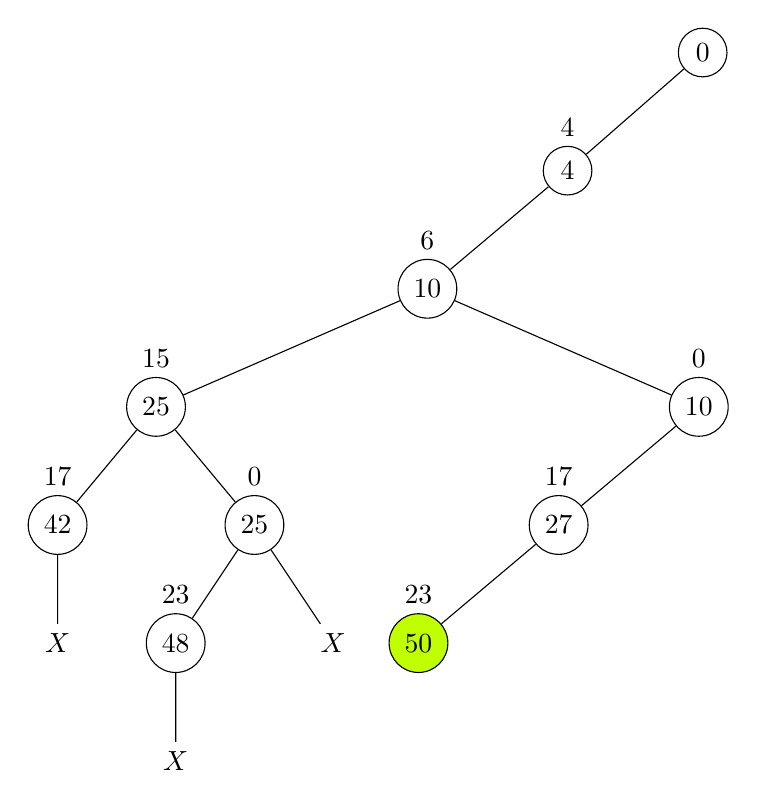
\begin{tikzpicture}[level/.style={sibling distance=100mm/#1}]
\node [circle,draw] (a){$0$}
  child {node [circle,draw, left=14mm, label = $4$] (b) {$4$}
      child {node [circle,draw, left=14mm, label = $6$] (c) {$10$}  
          child {node [circle,draw, left=14mm, label = $15$] (d) {$25$}
            child {node [circle,draw, label = $17$] (f) {$42$}
                child{node (1) {$X$}}
            }
            child {node [circle,draw, label = $0$] (g) {$25$}
                child {node [circle,draw, label = $23$] (h) {$48$}
                    child{node (1) {$X$}}
                }
                child{node (1) {$X$}}
            }
          }
          child {node [circle,draw, right=14mm, label = $0$] (e) {$10$}
              child {node [circle,draw, left=14mm, label = $17$] (i) {$27$}
                  child {node [circle,draw, left=14mm, fill = lime, label = $23$] (j) {$50$}
                  }
              }
          }
      }
  };
\end{tikzpicture}
\end{center}

As requested, we are only showing the path to the first combination that sums to 50.